\documentclass[1p]{elsarticle_modified}
%\bibliographystyle{elsarticle-num}

%\usepackage[colorlinks]{hyperref}
%\usepackage{abbrmath_seonhwa} %\Abb, \Ascr, \Acal ,\Abf, \Afrak
\usepackage{amsfonts}
\usepackage{amssymb}
\usepackage{amsmath}
\usepackage{amsthm}
\usepackage{scalefnt}
\usepackage{amsbsy}
\usepackage{kotex}
\usepackage{caption}
\usepackage{subfig}
\usepackage{color}
\usepackage{graphicx}
\usepackage{xcolor} %% white, black, red, green, blue, cyan, magenta, yellow
\usepackage{float}
\usepackage{setspace}
\usepackage{hyperref}

\usepackage{tikz}
\usetikzlibrary{arrows}

\usepackage{multirow}
\usepackage{array} % fixed length table
\usepackage{hhline}

%%%%%%%%%%%%%%%%%%%%%
\makeatletter
\renewcommand*\env@matrix[1][\arraystretch]{%
	\edef\arraystretch{#1}%
	\hskip -\arraycolsep
	\let\@ifnextchar\new@ifnextchar
	\array{*\c@MaxMatrixCols c}}
\makeatother %https://tex.stackexchange.com/questions/14071/how-can-i-increase-the-line-spacing-in-a-matrix
%%%%%%%%%%%%%%%

\usepackage[normalem]{ulem}

\newcommand{\msout}[1]{\ifmmode\text{\sout{\ensuremath{#1}}}\else\sout{#1}\fi}
%SOURCE: \msout is \stkout macro in https://tex.stackexchange.com/questions/20609/strikeout-in-math-mode

\newcommand{\cancel}[1]{
	\ifmmode
	{\color{red}\msout{#1}}
	\else
	{\color{red}\sout{#1}}
	\fi
}

\newcommand{\add}[1]{
	{\color{blue}\uwave{#1}}
}

\newcommand{\replace}[2]{
	\ifmmode
	{\color{red}\msout{#1}}{\color{blue}\uwave{#2}}
	\else
	{\color{red}\sout{#1}}{\color{blue}\uwave{#2}}
	\fi
}

\newcommand{\Sol}{\mathcal{S}} %segment
\newcommand{\D}{D} %diagram
\newcommand{\A}{\mathcal{A}} %arc


%%%%%%%%%%%%%%%%%%%%%%%%%%%%%5 test

\def\sl{\operatorname{\textup{SL}}(2,\Cbb)}
\def\psl{\operatorname{\textup{PSL}}(2,\Cbb)}
\def\quan{\mkern 1mu \triangleright \mkern 1mu}

\theoremstyle{definition}
\newtheorem{thm}{Theorem}[section]
\newtheorem{prop}[thm]{Proposition}
\newtheorem{lem}[thm]{Lemma}
\newtheorem{ques}[thm]{Question}
\newtheorem{cor}[thm]{Corollary}
\newtheorem{defn}[thm]{Definition}
\newtheorem{exam}[thm]{Example}
\newtheorem{rmk}[thm]{Remark}
\newtheorem{alg}[thm]{Algorithm}

\newcommand{\I}{\sqrt{-1}}
\begin{document}

%\begin{frontmatter}
%
%\title{Boundary parabolic representations of knots up to 8 crossings}
%
%%% Group authors per affiliation:
%\author{Yunhi Cho} 
%\address{Department of Mathematics, University of Seoul, Seoul, Korea}
%\ead{yhcho@uos.ac.kr}
%
%
%\author{Seonhwa Kim} %\fnref{s_kim}}
%\address{Center for Geometry and Physics, Institute for Basic Science, Pohang, 37673, Korea}
%\ead{ryeona17@ibs.re.kr}
%
%\author{Hyuk Kim}
%\address{Department of Mathematical Sciences, Seoul National University, Seoul 08826, Korea}
%\ead{hyukkim@snu.ac.kr}
%
%\author{Seokbeom Yoon}
%\address{Department of Mathematical Sciences, Seoul National University, Seoul, 08826,  Korea}
%\ead{sbyoon15@snu.ac.kr}
%
%\begin{abstract}
%We find all boundary parabolic representation of knots up to 8 crossings.
%
%\end{abstract}
%\begin{keyword}
%    \MSC[2010] 57M25 
%\end{keyword}
%
%\end{frontmatter}

%\linenumbers
%\tableofcontents
%
\newcommand\colored[1]{\textcolor{white}{\rule[-0.35ex]{0.8em}{1.4ex}}\kern-0.8em\color{red} #1}%
%\newcommand\colored[1]{\textcolor{white}{ #1}\kern-2.17ex	\textcolor{white}{ #1}\kern-1.81ex	\textcolor{white}{ #1}\kern-2.15ex\color{red}#1	}

{\Large $\underline{12n_{0362}~(K12n_{0362})}$}

\setlength{\tabcolsep}{10pt}
\renewcommand{\arraystretch}{1.6}
\vspace{1cm}\begin{tabular}{m{100pt}>{\centering\arraybackslash}m{274pt}}
\multirow{5}{120pt}{
	\centering
	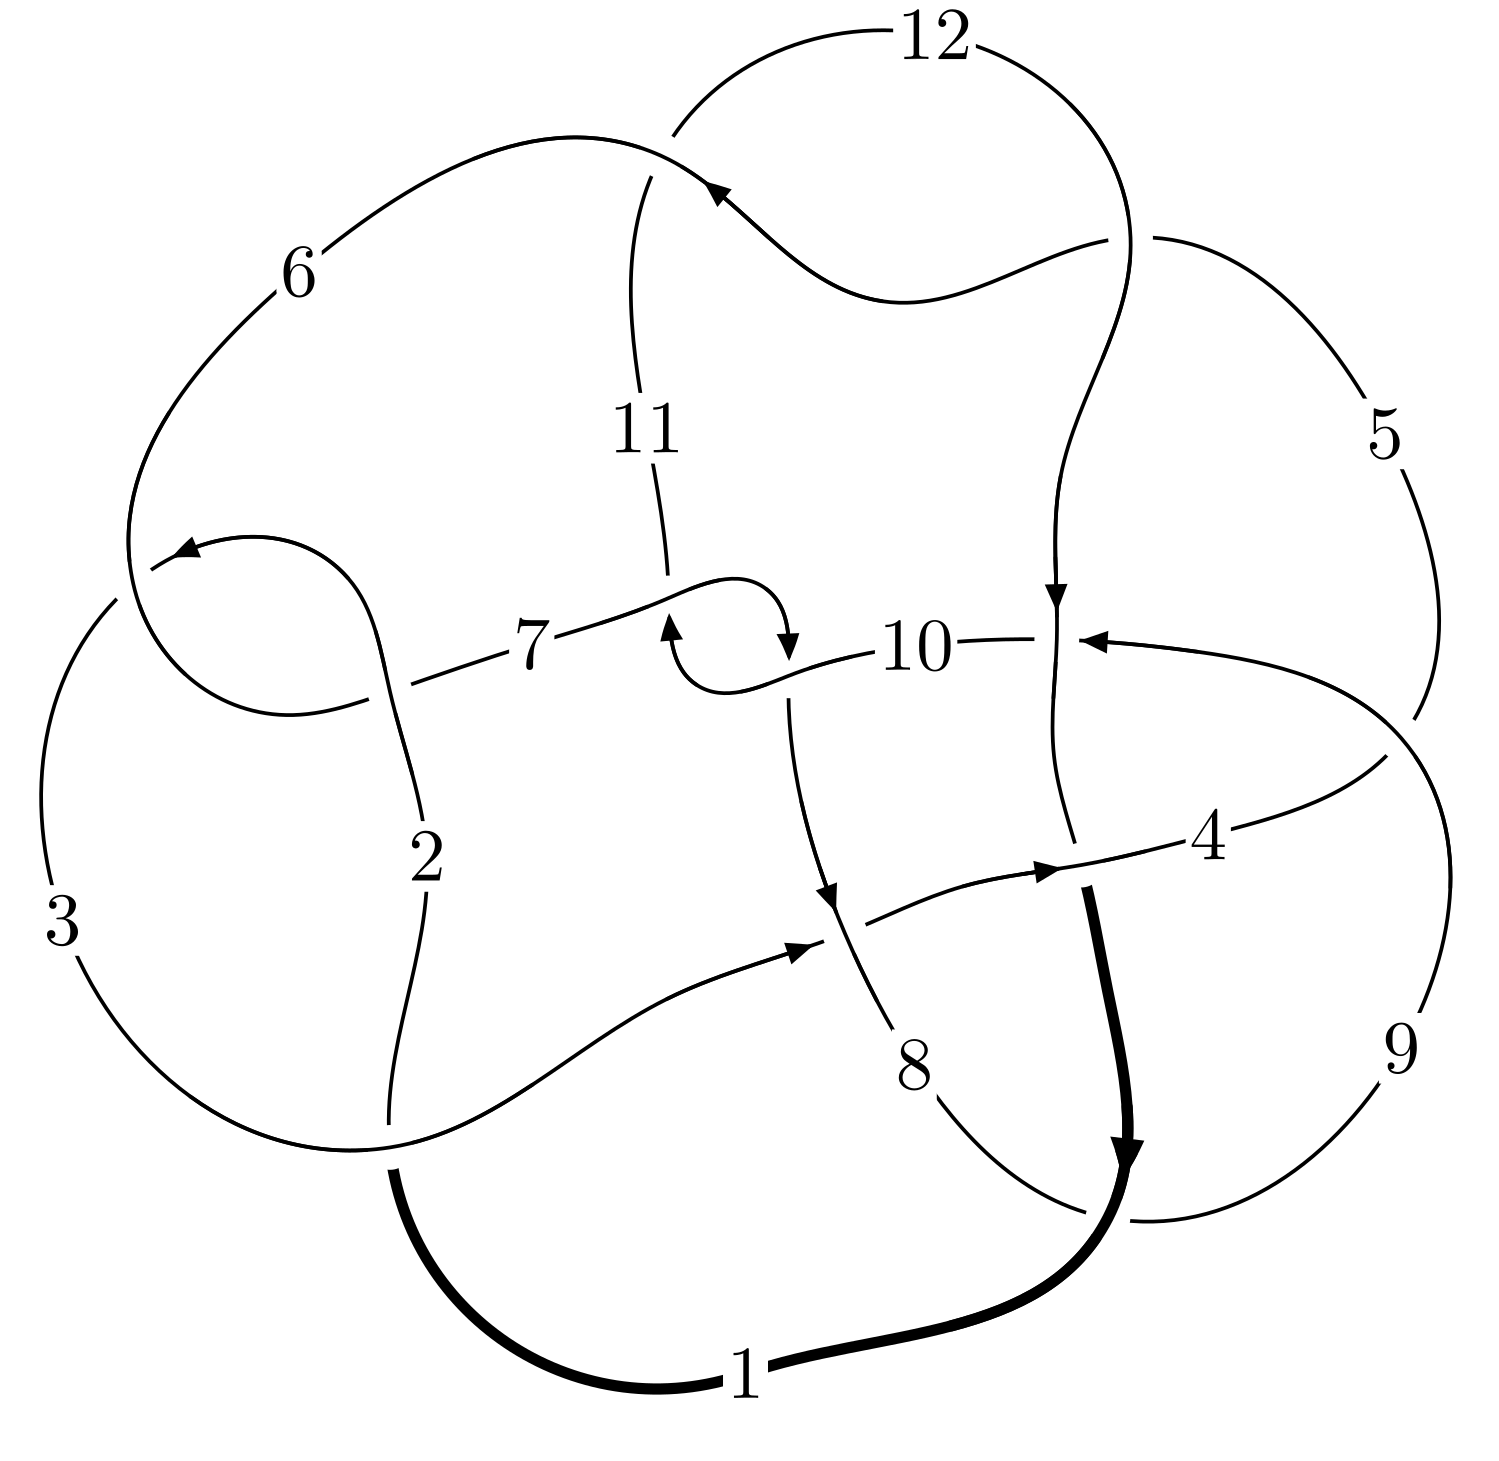
\includegraphics[width=112pt]{../../../GIT/diagram.site/Diagrams/png/2451_12n_0362.png}\\
\ \ \ A knot diagram\footnotemark}&
\allowdisplaybreaks
\textbf{Linearized knot diagam} \\
\cline{2-2}
 &
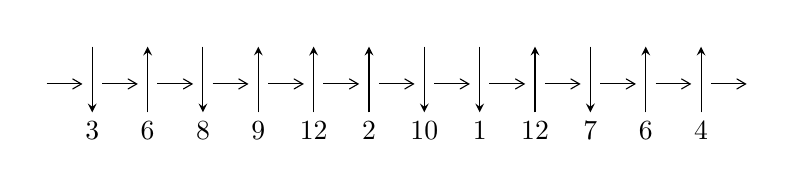
\begin{tikzpicture}[x=20pt, y=17pt]
	% nodes
	\node (C0) at (0, 0) {};
	\node (C1) at (1, 0) {};
	\node (C1U) at (1, +1) {};
	\node (C1D) at (1, -1) {3};

	\node (C2) at (2, 0) {};
	\node (C2U) at (2, +1) {};
	\node (C2D) at (2, -1) {6};

	\node (C3) at (3, 0) {};
	\node (C3U) at (3, +1) {};
	\node (C3D) at (3, -1) {8};

	\node (C4) at (4, 0) {};
	\node (C4U) at (4, +1) {};
	\node (C4D) at (4, -1) {9};

	\node (C5) at (5, 0) {};
	\node (C5U) at (5, +1) {};
	\node (C5D) at (5, -1) {12};

	\node (C6) at (6, 0) {};
	\node (C6U) at (6, +1) {};
	\node (C6D) at (6, -1) {2};

	\node (C7) at (7, 0) {};
	\node (C7U) at (7, +1) {};
	\node (C7D) at (7, -1) {10};

	\node (C8) at (8, 0) {};
	\node (C8U) at (8, +1) {};
	\node (C8D) at (8, -1) {1};

	\node (C9) at (9, 0) {};
	\node (C9U) at (9, +1) {};
	\node (C9D) at (9, -1) {12};

	\node (C10) at (10, 0) {};
	\node (C10U) at (10, +1) {};
	\node (C10D) at (10, -1) {7};

	\node (C11) at (11, 0) {};
	\node (C11U) at (11, +1) {};
	\node (C11D) at (11, -1) {6};

	\node (C12) at (12, 0) {};
	\node (C12U) at (12, +1) {};
	\node (C12D) at (12, -1) {4};
	\node (C13) at (13, 0) {};

	% arrows
	\draw[->,>={angle 60}]
	(C0) edge (C1) (C1) edge (C2) (C2) edge (C3) (C3) edge (C4) (C4) edge (C5) (C5) edge (C6) (C6) edge (C7) (C7) edge (C8) (C8) edge (C9) (C9) edge (C10) (C10) edge (C11) (C11) edge (C12) (C12) edge (C13) ;	\draw[->,>=stealth]
	(C1U) edge (C1D) (C2D) edge (C2U) (C3U) edge (C3D) (C4D) edge (C4U) (C5D) edge (C5U) (C6D) edge (C6U) (C7U) edge (C7D) (C8U) edge (C8D) (C9D) edge (C9U) (C10U) edge (C10D) (C11D) edge (C11U) (C12D) edge (C12U) ;
	\end{tikzpicture} \\
\hhline{~~} \\& 
\textbf{Solving Sequence} \\ \cline{2-2} 
 &
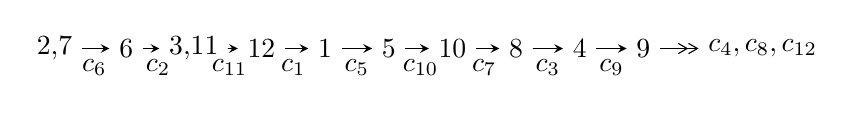
\begin{tikzpicture}[x=23pt, y=7pt]
	% node
	\node (A0) at (-1/8, 0) {2,7};
	\node (A1) at (1, 0) {6};
	\node (A2) at (33/16, 0) {3,11};
	\node (A3) at (25/8, 0) {12};
	\node (A4) at (33/8, 0) {1};
	\node (A5) at (41/8, 0) {5};
	\node (A6) at (49/8, 0) {10};
	\node (A7) at (57/8, 0) {8};
	\node (A8) at (65/8, 0) {4};
	\node (A9) at (73/8, 0) {9};
	\node (C1) at (1/2, -1) {$c_{6}$};
	\node (C2) at (3/2, -1) {$c_{2}$};
	\node (C3) at (21/8, -1) {$c_{11}$};
	\node (C4) at (29/8, -1) {$c_{1}$};
	\node (C5) at (37/8, -1) {$c_{5}$};
	\node (C6) at (45/8, -1) {$c_{10}$};
	\node (C7) at (53/8, -1) {$c_{7}$};
	\node (C8) at (61/8, -1) {$c_{3}$};
	\node (C9) at (69/8, -1) {$c_{9}$};
	\node (A10) at (11, 0) {$c_{4},c_{8},c_{12}$};

	% edge
	\draw[->,>=stealth]	
	(A0) edge (A1) (A1) edge (A2) (A2) edge (A3) (A3) edge (A4) (A4) edge (A5) (A5) edge (A6) (A6) edge (A7) (A7) edge (A8) (A8) edge (A9) ;
	\draw[->>,>={angle 60}]	
	(A9) edge (A10);
\end{tikzpicture} \\ 

\end{tabular} \\

\footnotetext{
The image of knot diagram is generated by the software ``\textbf{Draw programme}" developed by Andrew Bartholomew(\url{http://www.layer8.co.uk/maths/draw/index.htm\#Running-draw}), where we modified some parts for our purpose(\url{https://github.com/CATsTAILs/LinksPainter}).
}\phantom \\ \newline 
\centering \textbf{Ideals for irreducible components\footnotemark of $X_{\text{par}}$} 
 
\begin{align*}
I^u_{1}&=\langle 
6.22856\times10^{22} u^{28}+9.17947\times10^{22} u^{27}+\cdots+6.05360\times10^{22} b-3.78443\times10^{23},\\
\phantom{I^u_{1}}&\phantom{= \langle  }4.23380\times10^{22} u^{28}+6.00251\times10^{22} u^{27}+\cdots+1.81608\times10^{23} a-2.84140\times10^{23},\;u^{29}+u^{28}+\cdots-7 u+3\rangle \\
I^u_{2}&=\langle 
25 u^{13}+21 u^{12}+\cdots+38 b+39,\;28 u^{13}+22 u^{12}+\cdots+38 a+125,\\
\phantom{I^u_{2}}&\phantom{= \langle  }u^{14}+2 u^{12}+u^{11}+2 u^{10}+4 u^9+5 u^7+3 u^6+9 u^4-4 u^3+6 u^2- u+1\rangle \\
\\
\end{align*}
\raggedright * 2 irreducible components of $\dim_{\mathbb{C}}=0$, with total 43 representations.\\
\footnotetext{All coefficients of polynomials are rational numbers. But the coefficients are sometimes approximated in decimal forms when there is not enough margin.}
\newpage
\renewcommand{\arraystretch}{1}
\centering \section*{I. $I^u_{1}= \langle 6.23\times10^{22} u^{28}+9.18\times10^{22} u^{27}+\cdots+6.05\times10^{22} b-3.78\times10^{23},\;4.23\times10^{22} u^{28}+6.00\times10^{22} u^{27}+\cdots+1.82\times10^{23} a-2.84\times10^{23},\;u^{29}+u^{28}+\cdots-7 u+3 \rangle$}
\flushleft \textbf{(i) Arc colorings}\\
\begin{tabular}{m{7pt} m{180pt} m{7pt} m{180pt} }
\flushright $a_{2}=$&$\begin{pmatrix}0\\u\end{pmatrix}$ \\
\flushright $a_{7}=$&$\begin{pmatrix}1\\0\end{pmatrix}$ \\
\flushright $a_{6}=$&$\begin{pmatrix}1\\u^2\end{pmatrix}$ \\
\flushright $a_{3}=$&$\begin{pmatrix}u\\u^3+u\end{pmatrix}$ \\
\flushright $a_{11}=$&$\begin{pmatrix}-0.233129 u^{28}-0.330520 u^{27}+\cdots+0.142332 u+1.56458\\-1.02890 u^{28}-1.51637 u^{27}+\cdots-2.22286 u+6.25155\end{pmatrix}$ \\
\flushright $a_{12}=$&$\begin{pmatrix}-1.28168 u^{28}-1.86932 u^{27}+\cdots-2.09818 u+7.52395\\-1.33350 u^{28}-1.99028 u^{27}+\cdots-2.50900 u+7.72231\end{pmatrix}$ \\
\flushright $a_{1}=$&$\begin{pmatrix}u^3\\u^5+u^3+u\end{pmatrix}$ \\
\flushright $a_{5}=$&$\begin{pmatrix}-1.13087 u^{28}-1.69160 u^{27}+\cdots-3.73374 u+6.87479\\-0.452599 u^{28}-0.697647 u^{27}+\cdots-2.84372 u+2.78730\end{pmatrix}$ \\
\flushright $a_{10}=$&$\begin{pmatrix}-1.26203 u^{28}-1.84689 u^{27}+\cdots-2.08053 u+7.81613\\-1.02890 u^{28}-1.51637 u^{27}+\cdots-2.22286 u+6.25155\end{pmatrix}$ \\
\flushright $a_{8}=$&$\begin{pmatrix}-1.46451 u^{28}-2.20169 u^{27}+\cdots-3.99392 u+9.36262\\-0.583764 u^{28}-0.939441 u^{27}+\cdots-2.53644 u+3.54213\end{pmatrix}$ \\
\flushright $a_{4}=$&$\begin{pmatrix}1.44243 u^{28}+2.20325 u^{27}+\cdots+5.47310 u-7.92054\\0.146798 u^{28}+0.344443 u^{27}+\cdots+2.49249 u-0.145976\end{pmatrix}$ \\
\flushright $a_{9}=$&$\begin{pmatrix}-1.51831 u^{28}-2.23503 u^{27}+\cdots-3.75421 u+9.70241\\-0.975943 u^{28}-1.42608 u^{27}+\cdots-2.71519 u+6.24874\end{pmatrix}$\\&\end{tabular}
\flushleft \textbf{(ii) Obstruction class $= -1$}\\~\\
\flushleft \textbf{(iii) Cusp Shapes $= -\frac{284585492999900700617379}{60535961828035184424854} u^{28}-\frac{234964149766130199530131}{30267980914017592212427} u^{27}+\cdots-\frac{730227845218527654431241}{60535961828035184424854} u+\frac{888664531849357631011752}{30267980914017592212427}$}\\~\\
\newpage\renewcommand{\arraystretch}{1}
\flushleft \textbf{(iv) u-Polynomials at the component}\newline \\
\begin{tabular}{m{50pt}|m{274pt}}
Crossings & \hspace{64pt}u-Polynomials at each crossing \\
\hline $$\begin{aligned}c_{1}\end{aligned}$$&$\begin{aligned}
&u^{29}- u^{28}+\cdots+73 u-9
\end{aligned}$\\
\hline $$\begin{aligned}c_{2},c_{6}\end{aligned}$$&$\begin{aligned}
&u^{29}- u^{28}+\cdots-7 u-3
\end{aligned}$\\
\hline $$\begin{aligned}c_{3}\end{aligned}$$&$\begin{aligned}
&u^{29}+15 u^{25}+\cdots+32 u-11
\end{aligned}$\\
\hline $$\begin{aligned}c_{4}\end{aligned}$$&$\begin{aligned}
&u^{29}-24 u^{27}+\cdots-306 u-49
\end{aligned}$\\
\hline $$\begin{aligned}c_{5},c_{11}\end{aligned}$$&$\begin{aligned}
&u^{29}-3 u^{28}+\cdots-6023859 u-792917
\end{aligned}$\\
\hline $$\begin{aligned}c_{7},c_{10}\end{aligned}$$&$\begin{aligned}
&u^{29}-4 u^{28}+\cdots+590 u-1097
\end{aligned}$\\
\hline $$\begin{aligned}c_{8}\end{aligned}$$&$\begin{aligned}
&u^{29}- u^{28}+\cdots+2101 u-503
\end{aligned}$\\
\hline $$\begin{aligned}c_{9}\end{aligned}$$&$\begin{aligned}
&u^{29}+6 u^{28}+\cdots+8024 u-1461
\end{aligned}$\\
\hline $$\begin{aligned}c_{12}\end{aligned}$$&$\begin{aligned}
&u^{29}+2 u^{27}+\cdots+6 u+1
\end{aligned}$\\
\hline
\end{tabular}\\~\\
\newpage\renewcommand{\arraystretch}{1}
\flushleft \textbf{(v) Riley Polynomials at the component}\newline \\
\begin{tabular}{m{50pt}|m{274pt}}
Crossings & \hspace{64pt}Riley Polynomials at each crossing \\
\hline $$\begin{aligned}c_{1}\end{aligned}$$&$\begin{aligned}
&y^{29}+51 y^{28}+\cdots+1909 y-81
\end{aligned}$\\
\hline $$\begin{aligned}c_{2},c_{6}\end{aligned}$$&$\begin{aligned}
&y^{29}- y^{28}+\cdots+73 y-9
\end{aligned}$\\
\hline $$\begin{aligned}c_{3}\end{aligned}$$&$\begin{aligned}
&y^{29}+30 y^{27}+\cdots-538 y-121
\end{aligned}$\\
\hline $$\begin{aligned}c_{4}\end{aligned}$$&$\begin{aligned}
&y^{29}-48 y^{28}+\cdots+26604 y-2401
\end{aligned}$\\
\hline $$\begin{aligned}c_{5},c_{11}\end{aligned}$$&$\begin{aligned}
&y^{29}-99 y^{28}+\cdots+5243889665927 y-628717368889
\end{aligned}$\\
\hline $$\begin{aligned}c_{7},c_{10}\end{aligned}$$&$\begin{aligned}
&y^{29}+50 y^{28}+\cdots+4466238 y-1203409
\end{aligned}$\\
\hline $$\begin{aligned}c_{8}\end{aligned}$$&$\begin{aligned}
&y^{29}+31 y^{28}+\cdots-4491917 y-253009
\end{aligned}$\\
\hline $$\begin{aligned}c_{9}\end{aligned}$$&$\begin{aligned}
&y^{29}-62 y^{28}+\cdots-12595514 y-2134521
\end{aligned}$\\
\hline $$\begin{aligned}c_{12}\end{aligned}$$&$\begin{aligned}
&y^{29}+4 y^{28}+\cdots+12 y-1
\end{aligned}$\\
\hline
\end{tabular}\\~\\
\newpage\flushleft \textbf{(vi) Complex Volumes and Cusp Shapes}
$$\begin{array}{c|c|c}  
\text{Solutions to }I^u_{1}& \I (\text{vol} + \sqrt{-1}CS) & \text{Cusp shape}\\
 \hline 
\begin{aligned}
u &= -0.373209 + 0.987492 I \\
a &= -0.104866 - 0.390683 I \\
b &= \phantom{-}0.354634 + 0.496131 I\end{aligned}
 & -0.91018 - 2.91066 I & \phantom{-}5.01825 + 3.66237 I \\ \hline\begin{aligned}
u &= -0.373209 - 0.987492 I \\
a &= -0.104866 + 0.390683 I \\
b &= \phantom{-}0.354634 - 0.496131 I\end{aligned}
 & -0.91018 + 2.91066 I & \phantom{-}5.01825 - 3.66237 I \\ \hline\begin{aligned}
u &= -0.676723 + 0.657927 I \\
a &= \phantom{-}1.37413 - 1.24981 I \\
b &= -0.587705 - 0.859816 I\end{aligned}
 & \phantom{-}3.33766 - 4.86187 I & \phantom{-}6.31556 + 7.79080 I \\ \hline\begin{aligned}
u &= -0.676723 - 0.657927 I \\
a &= \phantom{-}1.37413 + 1.24981 I \\
b &= -0.587705 + 0.859816 I\end{aligned}
 & \phantom{-}3.33766 + 4.86187 I & \phantom{-}6.31556 - 7.79080 I \\ \hline\begin{aligned}
u &= -1.003850 + 0.405083 I \\
a &= \phantom{-}0.881641 - 0.955047 I \\
b &= -1.52183 + 1.81794 I\end{aligned}
 & \phantom{-}4.69261 + 0.54758 I & \phantom{-}8.30748 - 0.23720 I \\ \hline\begin{aligned}
u &= -1.003850 - 0.405083 I \\
a &= \phantom{-}0.881641 + 0.955047 I \\
b &= -1.52183 - 1.81794 I\end{aligned}
 & \phantom{-}4.69261 - 0.54758 I & \phantom{-}8.30748 + 0.23720 I \\ \hline\begin{aligned}
u &= \phantom{-}0.690839 + 0.852823 I \\
a &= -1.58706 - 0.12680 I \\
b &= \phantom{-}1.168090 - 0.519664 I\end{aligned}
 & -1.72733 + 5.06544 I & -0.06902 - 8.02609 I \\ \hline\begin{aligned}
u &= \phantom{-}0.690839 - 0.852823 I \\
a &= -1.58706 + 0.12680 I \\
b &= \phantom{-}1.168090 + 0.519664 I\end{aligned}
 & -1.72733 - 5.06544 I & -0.06902 + 8.02609 I \\ \hline\begin{aligned}
u &= \phantom{-}0.301765 + 1.063800 I \\
a &= \phantom{-}0.115276 - 1.216510 I \\
b &= \phantom{-}0.350185 + 0.484209 I\end{aligned}
 & -3.69483 + 0.73314 I & -5.00047 + 1.33936 I \\ \hline\begin{aligned}
u &= \phantom{-}0.301765 - 1.063800 I \\
a &= \phantom{-}0.115276 + 1.216510 I \\
b &= \phantom{-}0.350185 - 0.484209 I\end{aligned}
 & -3.69483 - 0.73314 I & -5.00047 - 1.33936 I\\
 \hline 
 \end{array}$$\newpage$$\begin{array}{c|c|c}  
\text{Solutions to }I^u_{1}& \I (\text{vol} + \sqrt{-1}CS) & \text{Cusp shape}\\
 \hline 
\begin{aligned}
u &= \phantom{-}0.746264 + 0.430998 I \\
a &= \phantom{-}0.459246 + 0.593245 I \\
b &= -1.06802 - 1.95662 I\end{aligned}
 & \phantom{-}4.83649 + 4.86751 I & \phantom{-}7.86120 - 7.38894 I \\ \hline\begin{aligned}
u &= \phantom{-}0.746264 - 0.430998 I \\
a &= \phantom{-}0.459246 - 0.593245 I \\
b &= -1.06802 + 1.95662 I\end{aligned}
 & \phantom{-}4.83649 - 4.86751 I & \phantom{-}7.86120 + 7.38894 I \\ \hline\begin{aligned}
u &= -1.17492\phantom{ +0.000000I} \\
a &= \phantom{-}1.30562\phantom{ +0.000000I} \\
b &= -1.24715\phantom{ +0.000000I}\end{aligned}
 & \phantom{-}2.83868\phantom{ +0.000000I} & -0.284290\phantom{ +0.000000I} \\ \hline\begin{aligned}
u &= \phantom{-}0.785504 + 0.193075 I \\
a &= -0.69313 + 1.26338 I \\
b &= \phantom{-}0.123042 + 0.893877 I\end{aligned}
 & \phantom{-}5.21089 - 2.34623 I & \phantom{-}11.13604 + 2.03452 I \\ \hline\begin{aligned}
u &= \phantom{-}0.785504 - 0.193075 I \\
a &= -0.69313 - 1.26338 I \\
b &= \phantom{-}0.123042 - 0.893877 I\end{aligned}
 & \phantom{-}5.21089 + 2.34623 I & \phantom{-}11.13604 - 2.03452 I \\ \hline\begin{aligned}
u &= -0.636133 + 0.449347 I \\
a &= \phantom{-}0.946998 - 0.046552 I \\
b &= -0.353642 - 0.116483 I\end{aligned}
 & \phantom{-}1.14437 - 0.87641 I & \phantom{-}6.31209 + 2.91044 I \\ \hline\begin{aligned}
u &= -0.636133 - 0.449347 I \\
a &= \phantom{-}0.946998 + 0.046552 I \\
b &= -0.353642 + 0.116483 I\end{aligned}
 & \phantom{-}1.14437 + 0.87641 I & \phantom{-}6.31209 - 2.91044 I \\ \hline\begin{aligned}
u &= -0.193861 + 0.669195 I \\
a &= -1.12680 - 1.16765 I \\
b &= \phantom{-}0.873432 + 0.640443 I\end{aligned}
 & -1.76493 - 2.37343 I & -1.52317 + 0.50273 I \\ \hline\begin{aligned}
u &= -0.193861 - 0.669195 I \\
a &= -1.12680 + 1.16765 I \\
b &= \phantom{-}0.873432 - 0.640443 I\end{aligned}
 & -1.76493 + 2.37343 I & -1.52317 - 0.50273 I \\ \hline\begin{aligned}
u &= \phantom{-}0.510226 + 0.048164 I \\
a &= \phantom{-}0.823085 - 0.113650 I \\
b &= \phantom{-}0.302073 - 0.906163 I\end{aligned}
 & -0.71888 + 2.03179 I & \phantom{-}1.45662 - 4.22219 I\\
 \hline 
 \end{array}$$\newpage$$\begin{array}{c|c|c}  
\text{Solutions to }I^u_{1}& \I (\text{vol} + \sqrt{-1}CS) & \text{Cusp shape}\\
 \hline 
\begin{aligned}
u &= \phantom{-}0.510226 - 0.048164 I \\
a &= \phantom{-}0.823085 + 0.113650 I \\
b &= \phantom{-}0.302073 + 0.906163 I\end{aligned}
 & -0.71888 - 2.03179 I & \phantom{-}1.45662 + 4.22219 I \\ \hline\begin{aligned}
u &= \phantom{-}1.15086 + 1.05205 I \\
a &= \phantom{-}1.35233 - 1.13268 I \\
b &= -0.61827 + 2.28433 I\end{aligned}
 & \phantom{-}17.8200 + 4.6744 I & \phantom{-}4.90361 - 1.93865 I \\ \hline\begin{aligned}
u &= \phantom{-}1.15086 - 1.05205 I \\
a &= \phantom{-}1.35233 + 1.13268 I \\
b &= -0.61827 - 2.28433 I\end{aligned}
 & \phantom{-}17.8200 - 4.6744 I & \phantom{-}4.90361 + 1.93865 I \\ \hline\begin{aligned}
u &= \phantom{-}1.06456 + 1.14906 I \\
a &= -1.02725 + 1.45432 I \\
b &= \phantom{-}0.02209 - 2.23942 I\end{aligned}
 & \phantom{-}17.4581 + 3.4840 I & \phantom{-}4.59551 - 2.22003 I \\ \hline\begin{aligned}
u &= \phantom{-}1.06456 - 1.14906 I \\
a &= -1.02725 - 1.45432 I \\
b &= \phantom{-}0.02209 + 2.23942 I\end{aligned}
 & \phantom{-}17.4581 - 3.4840 I & \phantom{-}4.59551 + 2.22003 I \\ \hline\begin{aligned}
u &= -1.14088 + 1.11108 I \\
a &= \phantom{-}1.45432 + 1.41280 I \\
b &= -0.63801 - 2.49907 I\end{aligned}
 & \phantom{-}17.2047 - 12.2799 I & \phantom{-}4.10699 + 5.81074 I \\ \hline\begin{aligned}
u &= -1.14088 - 1.11108 I \\
a &= \phantom{-}1.45432 - 1.41280 I \\
b &= -0.63801 + 2.49907 I\end{aligned}
 & \phantom{-}17.2047 + 12.2799 I & \phantom{-}4.10699 - 5.81074 I \\ \hline\begin{aligned}
u &= -1.13790 + 1.15169 I \\
a &= -1.18740 - 1.61441 I \\
b &= \phantom{-}0.21751 + 2.42455 I\end{aligned}
 & \phantom{-}17.1162 + 3.8820 I & \phantom{-}4.22145 - 2.11285 I \\ \hline\begin{aligned}
u &= -1.13790 - 1.15169 I \\
a &= -1.18740 + 1.61441 I \\
b &= \phantom{-}0.21751 - 2.42455 I\end{aligned}
 & \phantom{-}17.1162 - 3.8820 I & \phantom{-}4.22145 + 2.11285 I\\
 \hline 
 \end{array}$$\newpage\newpage\renewcommand{\arraystretch}{1}
\centering \section*{II. $I^u_{2}= \langle 25 u^{13}+21 u^{12}+\cdots+38 b+39,\;28 u^{13}+22 u^{12}+\cdots+38 a+125,\;u^{14}+2 u^{12}+\cdots- u+1 \rangle$}
\flushleft \textbf{(i) Arc colorings}\\
\begin{tabular}{m{7pt} m{180pt} m{7pt} m{180pt} }
\flushright $a_{2}=$&$\begin{pmatrix}0\\u\end{pmatrix}$ \\
\flushright $a_{7}=$&$\begin{pmatrix}1\\0\end{pmatrix}$ \\
\flushright $a_{6}=$&$\begin{pmatrix}1\\u^2\end{pmatrix}$ \\
\flushright $a_{3}=$&$\begin{pmatrix}u\\u^3+u\end{pmatrix}$ \\
\flushright $a_{11}=$&$\begin{pmatrix}-0.736842 u^{13}-0.578947 u^{12}+\cdots-0.0789474 u-3.28947\\-0.657895 u^{13}-0.552632 u^{12}+\cdots-2.05263 u-1.02632\end{pmatrix}$ \\
\flushright $a_{12}=$&$\begin{pmatrix}-1.86842 u^{13}-1.28947 u^{12}+\cdots-2.28947 u-4.89474\\-0.394737 u^{13}-0.131579 u^{12}+\cdots-1.63158 u-0.315789\end{pmatrix}$ \\
\flushright $a_{1}=$&$\begin{pmatrix}u^3\\u^5+u^3+u\end{pmatrix}$ \\
\flushright $a_{5}=$&$\begin{pmatrix}3.65789 u^{13}+1.55263 u^{12}+\cdots+7.55263 u+6.52632\\-\frac{1}{2} u^9+u^8+\cdots+\frac{3}{2} u-\frac{1}{2}\end{pmatrix}$ \\
\flushright $a_{10}=$&$\begin{pmatrix}-1.39474 u^{13}-1.13158 u^{12}+\cdots-2.13158 u-4.31579\\-0.657895 u^{13}-0.552632 u^{12}+\cdots-2.05263 u-1.02632\end{pmatrix}$ \\
\flushright $a_{8}=$&$\begin{pmatrix}2.02632 u^{13}+0.342105 u^{12}+\cdots+6.34211 u+1.92105\\0.921053 u^{13}-0.526316 u^{12}+\cdots+2.47368 u-1.26316\end{pmatrix}$ \\
\flushright $a_{4}=$&$\begin{pmatrix}-0.315789 u^{13}+0.894737 u^{12}+\cdots-6.10526 u+4.44737\\1.15789 u^{13}+0.0526316 u^{12}+\cdots+2.55263 u-0.473684\end{pmatrix}$ \\
\flushright $a_{9}=$&$\begin{pmatrix}2.21053 u^{13}+0.736842 u^{12}+\cdots+6.73684 u+2.36842\\0.394737 u^{13}-0.868421 u^{12}+\cdots+1.13158 u-1.68421\end{pmatrix}$\\&\end{tabular}
\flushleft \textbf{(ii) Obstruction class $= 1$}\\~\\
\flushleft \textbf{(iii) Cusp Shapes $= \frac{275}{38} u^{13}+\frac{117}{38} u^{12}+10 u^{11}+\frac{389}{38} u^{10}+\frac{191}{19} u^9+\frac{993}{38} u^8+\frac{61}{19} u^7+\frac{643}{38} u^6+\frac{1071}{38} u^5-\frac{175}{38} u^4+\frac{1549}{38} u^3-\frac{105}{19} u^2+\frac{49}{19} u+\frac{201}{38}$}\\~\\
\newpage\renewcommand{\arraystretch}{1}
\flushleft \textbf{(iv) u-Polynomials at the component}\newline \\
\begin{tabular}{m{50pt}|m{274pt}}
Crossings & \hspace{64pt}u-Polynomials at each crossing \\
\hline $$\begin{aligned}c_{1}\end{aligned}$$&$\begin{aligned}
&u^{14}-4 u^{13}+\cdots-11 u+1
\end{aligned}$\\
\hline $$\begin{aligned}c_{2}\end{aligned}$$&$\begin{aligned}
&u^{14}+2 u^{12}- u^{11}+2 u^{10}-4 u^9-5 u^7+3 u^6+9 u^4+4 u^3+6 u^2+u+1
\end{aligned}$\\
\hline $$\begin{aligned}c_{3}\end{aligned}$$&$\begin{aligned}
&u^{14}- u^{13}-3 u^{12}+4 u^{11}+4 u^{10}-7 u^9+6 u^7-6 u^6-2 u^5+9 u^4-5 u^2+1
\end{aligned}$\\
\hline $$\begin{aligned}c_{4}\end{aligned}$$&$\begin{aligned}
&u^{14}+u^{13}+\cdots-8 u+1
\end{aligned}$\\
\hline $$\begin{aligned}c_{5}\end{aligned}$$&$\begin{aligned}
&u^{14}+2 u^{13}+\cdots-9 u+1
\end{aligned}$\\
\hline $$\begin{aligned}c_{6}\end{aligned}$$&$\begin{aligned}
&u^{14}+2 u^{12}+u^{11}+2 u^{10}+4 u^9+5 u^7+3 u^6+9 u^4-4 u^3+6 u^2- u+1
\end{aligned}$\\
\hline $$\begin{aligned}c_{7}\end{aligned}$$&$\begin{aligned}
&u^{14}+u^{13}+\cdots+2 u+1
\end{aligned}$\\
\hline $$\begin{aligned}c_{8}\end{aligned}$$&$\begin{aligned}
&u^{14}+6 u^{13}+\cdots+3 u+1
\end{aligned}$\\
\hline $$\begin{aligned}c_{9}\end{aligned}$$&$\begin{aligned}
&u^{14}+15 u^{13}+\cdots+430 u+67
\end{aligned}$\\
\hline $$\begin{aligned}c_{10}\end{aligned}$$&$\begin{aligned}
&u^{14}- u^{13}+\cdots-2 u+1
\end{aligned}$\\
\hline $$\begin{aligned}c_{11}\end{aligned}$$&$\begin{aligned}
&u^{14}-2 u^{13}+\cdots+9 u+1
\end{aligned}$\\
\hline $$\begin{aligned}c_{12}\end{aligned}$$&$\begin{aligned}
&u^{14}+u^{13}+\cdots+4 u^2+1
\end{aligned}$\\
\hline
\end{tabular}\\~\\
\newpage\renewcommand{\arraystretch}{1}
\flushleft \textbf{(v) Riley Polynomials at the component}\newline \\
\begin{tabular}{m{50pt}|m{274pt}}
Crossings & \hspace{64pt}Riley Polynomials at each crossing \\
\hline $$\begin{aligned}c_{1}\end{aligned}$$&$\begin{aligned}
&y^{14}+12 y^{12}+\cdots-29 y+1
\end{aligned}$\\
\hline $$\begin{aligned}c_{2},c_{6}\end{aligned}$$&$\begin{aligned}
&y^{14}+4 y^{13}+\cdots+11 y+1
\end{aligned}$\\
\hline $$\begin{aligned}c_{3}\end{aligned}$$&$\begin{aligned}
&y^{14}-7 y^{13}+\cdots-10 y+1
\end{aligned}$\\
\hline $$\begin{aligned}c_{4}\end{aligned}$$&$\begin{aligned}
&y^{14}-15 y^{13}+\cdots-36 y+1
\end{aligned}$\\
\hline $$\begin{aligned}c_{5},c_{11}\end{aligned}$$&$\begin{aligned}
&y^{14}+2 y^{13}+\cdots-3 y+1
\end{aligned}$\\
\hline $$\begin{aligned}c_{7},c_{10}\end{aligned}$$&$\begin{aligned}
&y^{14}+3 y^{13}+\cdots+2 y+1
\end{aligned}$\\
\hline $$\begin{aligned}c_{8}\end{aligned}$$&$\begin{aligned}
&y^{14}+12 y^{13}+\cdots+5 y+1
\end{aligned}$\\
\hline $$\begin{aligned}c_{9}\end{aligned}$$&$\begin{aligned}
&y^{14}-13 y^{13}+\cdots+12482 y+4489
\end{aligned}$\\
\hline $$\begin{aligned}c_{12}\end{aligned}$$&$\begin{aligned}
&y^{14}+5 y^{13}+\cdots+8 y+1
\end{aligned}$\\
\hline
\end{tabular}\\~\\
\newpage\flushleft \textbf{(vi) Complex Volumes and Cusp Shapes}
$$\begin{array}{c|c|c}  
\text{Solutions to }I^u_{2}& \I (\text{vol} + \sqrt{-1}CS) & \text{Cusp shape}\\
 \hline 
\begin{aligned}
u &= -0.083441 + 1.078120 I \\
a &= -0.61041 - 1.75239 I \\
b &= \phantom{-}0.359465 + 0.927829 I\end{aligned}
 & -3.38940 - 1.96463 I & -3.36465 + 3.16114 I \\ \hline\begin{aligned}
u &= -0.083441 - 1.078120 I \\
a &= -0.61041 + 1.75239 I \\
b &= \phantom{-}0.359465 - 0.927829 I\end{aligned}
 & -3.38940 + 1.96463 I & -3.36465 - 3.16114 I \\ \hline\begin{aligned}
u &= \phantom{-}0.897543 + 0.628482 I \\
a &= -0.569463 - 0.217274 I \\
b &= \phantom{-}0.362370 - 1.134100 I\end{aligned}
 & \phantom{-}2.05951 + 4.06327 I & \phantom{-}2.33224 - 4.24956 I \\ \hline\begin{aligned}
u &= \phantom{-}0.897543 - 0.628482 I \\
a &= -0.569463 + 0.217274 I \\
b &= \phantom{-}0.362370 + 1.134100 I\end{aligned}
 & \phantom{-}2.05951 - 4.06327 I & \phantom{-}2.33224 + 4.24956 I \\ \hline\begin{aligned}
u &= \phantom{-}0.330516 + 0.759270 I \\
a &= -1.019620 + 0.347965 I \\
b &= \phantom{-}0.931938 - 0.797201 I\end{aligned}
 & -1.80322 + 3.24685 I & -4.21171 - 8.28864 I \\ \hline\begin{aligned}
u &= \phantom{-}0.330516 - 0.759270 I \\
a &= -1.019620 - 0.347965 I \\
b &= \phantom{-}0.931938 + 0.797201 I\end{aligned}
 & -1.80322 - 3.24685 I & -4.21171 + 8.28864 I \\ \hline\begin{aligned}
u &= \phantom{-}0.605820 + 1.045230 I \\
a &= \phantom{-}0.540931 - 0.356236 I \\
b &= \phantom{-}0.280794 + 0.717818 I\end{aligned}
 & \phantom{-}0.55352 + 1.43715 I & \phantom{-}2.87679 - 0.95272 I \\ \hline\begin{aligned}
u &= \phantom{-}0.605820 - 1.045230 I \\
a &= \phantom{-}0.540931 + 0.356236 I \\
b &= \phantom{-}0.280794 - 0.717818 I\end{aligned}
 & \phantom{-}0.55352 - 1.43715 I & \phantom{-}2.87679 + 0.95272 I \\ \hline\begin{aligned}
u &= -1.201470 + 0.299412 I \\
a &= \phantom{-}0.998346 - 0.558650 I \\
b &= -1.21886 + 1.14220 I\end{aligned}
 & \phantom{-}3.33918 + 0.87099 I & \phantom{-}2.89094 - 4.11825 I \\ \hline\begin{aligned}
u &= -1.201470 - 0.299412 I \\
a &= \phantom{-}0.998346 + 0.558650 I \\
b &= -1.21886 - 1.14220 I\end{aligned}
 & \phantom{-}3.33918 - 0.87099 I & \phantom{-}2.89094 + 4.11825 I\\
 \hline 
 \end{array}$$\newpage$$\begin{array}{c|c|c}  
\text{Solutions to }I^u_{2}& \I (\text{vol} + \sqrt{-1}CS) & \text{Cusp shape}\\
 \hline 
\begin{aligned}
u &= -0.555233 + 1.209370 I \\
a &= \phantom{-}1.330610 - 0.277547 I \\
b &= -0.600887 - 0.417434 I\end{aligned}
 & \phantom{-}0.03234 - 6.71387 I & \phantom{-}0.87198 + 7.20748 I \\ \hline\begin{aligned}
u &= -0.555233 - 1.209370 I \\
a &= \phantom{-}1.330610 + 0.277547 I \\
b &= -0.600887 + 0.417434 I\end{aligned}
 & \phantom{-}0.03234 + 6.71387 I & \phantom{-}0.87198 - 7.20748 I \\ \hline\begin{aligned}
u &= \phantom{-}0.006261 + 0.511967 I \\
a &= -2.67040 + 0.41495 I \\
b &= -0.614823 - 0.394790 I\end{aligned}
 & \phantom{-}4.14287 + 3.38328 I & \phantom{-}6.10441 - 3.17614 I \\ \hline\begin{aligned}
u &= \phantom{-}0.006261 - 0.511967 I \\
a &= -2.67040 - 0.41495 I \\
b &= -0.614823 + 0.394790 I\end{aligned}
 & \phantom{-}4.14287 - 3.38328 I & \phantom{-}6.10441 + 3.17614 I\\
 \hline 
 \end{array}$$\newpage
\newpage\renewcommand{\arraystretch}{1}
\centering \section*{ III. u-Polynomials}
\begin{tabular}{m{50pt}|m{274pt}}
Crossings & \hspace{64pt}u-Polynomials at each crossing \\
\hline $$\begin{aligned}c_{1}\end{aligned}$$&$\begin{aligned}
&(u^{14}-4 u^{13}+\cdots-11 u+1)(u^{29}- u^{28}+\cdots+73 u-9)
\end{aligned}$\\
\hline $$\begin{aligned}c_{2}\end{aligned}$$&$\begin{aligned}
&(u^{14}+2 u^{12}- u^{11}+2 u^{10}-4 u^9-5 u^7+3 u^6+9 u^4+4 u^3+6 u^2+u+1)\\
&\cdot(u^{29}- u^{28}+\cdots-7 u-3)
\end{aligned}$\\
\hline $$\begin{aligned}c_{3}\end{aligned}$$&$\begin{aligned}
&(u^{14}- u^{13}-3 u^{12}+4 u^{11}+4 u^{10}-7 u^9+6 u^7-6 u^6-2 u^5+9 u^4-5 u^2+1)\\
&\cdot(u^{29}+15 u^{25}+\cdots+32 u-11)
\end{aligned}$\\
\hline $$\begin{aligned}c_{4}\end{aligned}$$&$\begin{aligned}
&(u^{14}+u^{13}+\cdots-8 u+1)(u^{29}-24 u^{27}+\cdots-306 u-49)
\end{aligned}$\\
\hline $$\begin{aligned}c_{5}\end{aligned}$$&$\begin{aligned}
&(u^{14}+2 u^{13}+\cdots-9 u+1)(u^{29}-3 u^{28}+\cdots-6023859 u-792917)
\end{aligned}$\\
\hline $$\begin{aligned}c_{6}\end{aligned}$$&$\begin{aligned}
&(u^{14}+2 u^{12}+u^{11}+2 u^{10}+4 u^9+5 u^7+3 u^6+9 u^4-4 u^3+6 u^2- u+1)\\
&\cdot(u^{29}- u^{28}+\cdots-7 u-3)
\end{aligned}$\\
\hline $$\begin{aligned}c_{7}\end{aligned}$$&$\begin{aligned}
&(u^{14}+u^{13}+\cdots+2 u+1)(u^{29}-4 u^{28}+\cdots+590 u-1097)
\end{aligned}$\\
\hline $$\begin{aligned}c_{8}\end{aligned}$$&$\begin{aligned}
&(u^{14}+6 u^{13}+\cdots+3 u+1)(u^{29}- u^{28}+\cdots+2101 u-503)
\end{aligned}$\\
\hline $$\begin{aligned}c_{9}\end{aligned}$$&$\begin{aligned}
&(u^{14}+15 u^{13}+\cdots+430 u+67)(u^{29}+6 u^{28}+\cdots+8024 u-1461)
\end{aligned}$\\
\hline $$\begin{aligned}c_{10}\end{aligned}$$&$\begin{aligned}
&(u^{14}- u^{13}+\cdots-2 u+1)(u^{29}-4 u^{28}+\cdots+590 u-1097)
\end{aligned}$\\
\hline $$\begin{aligned}c_{11}\end{aligned}$$&$\begin{aligned}
&(u^{14}-2 u^{13}+\cdots+9 u+1)(u^{29}-3 u^{28}+\cdots-6023859 u-792917)
\end{aligned}$\\
\hline $$\begin{aligned}c_{12}\end{aligned}$$&$\begin{aligned}
&(u^{14}+u^{13}+\cdots+4 u^2+1)(u^{29}+2 u^{27}+\cdots+6 u+1)
\end{aligned}$\\
\hline
\end{tabular}\newpage\renewcommand{\arraystretch}{1}
\centering \section*{ IV. Riley Polynomials}
\begin{tabular}{m{50pt}|m{274pt}}
Crossings & \hspace{64pt}Riley Polynomials at each crossing \\
\hline $$\begin{aligned}c_{1}\end{aligned}$$&$\begin{aligned}
&(y^{14}+12 y^{12}+\cdots-29 y+1)(y^{29}+51 y^{28}+\cdots+1909 y-81)
\end{aligned}$\\
\hline $$\begin{aligned}c_{2},c_{6}\end{aligned}$$&$\begin{aligned}
&(y^{14}+4 y^{13}+\cdots+11 y+1)(y^{29}- y^{28}+\cdots+73 y-9)
\end{aligned}$\\
\hline $$\begin{aligned}c_{3}\end{aligned}$$&$\begin{aligned}
&(y^{14}-7 y^{13}+\cdots-10 y+1)(y^{29}+30 y^{27}+\cdots-538 y-121)
\end{aligned}$\\
\hline $$\begin{aligned}c_{4}\end{aligned}$$&$\begin{aligned}
&(y^{14}-15 y^{13}+\cdots-36 y+1)(y^{29}-48 y^{28}+\cdots+26604 y-2401)
\end{aligned}$\\
\hline $$\begin{aligned}c_{5},c_{11}\end{aligned}$$&$\begin{aligned}
&(y^{14}+2 y^{13}+\cdots-3 y+1)\\
&\cdot(y^{29}-99 y^{28}+\cdots+5243889665927 y-628717368889)
\end{aligned}$\\
\hline $$\begin{aligned}c_{7},c_{10}\end{aligned}$$&$\begin{aligned}
&(y^{14}+3 y^{13}+\cdots+2 y+1)(y^{29}+50 y^{28}+\cdots+4466238 y-1203409)
\end{aligned}$\\
\hline $$\begin{aligned}c_{8}\end{aligned}$$&$\begin{aligned}
&(y^{14}+12 y^{13}+\cdots+5 y+1)(y^{29}+31 y^{28}+\cdots-4491917 y-253009)
\end{aligned}$\\
\hline $$\begin{aligned}c_{9}\end{aligned}$$&$\begin{aligned}
&(y^{14}-13 y^{13}+\cdots+12482 y+4489)\\
&\cdot(y^{29}-62 y^{28}+\cdots-12595514 y-2134521)
\end{aligned}$\\
\hline $$\begin{aligned}c_{12}\end{aligned}$$&$\begin{aligned}
&(y^{14}+5 y^{13}+\cdots+8 y+1)(y^{29}+4 y^{28}+\cdots+12 y-1)
\end{aligned}$\\
\hline
\end{tabular}
\vskip 2pc
\end{document}